\documentclass[journal,12pt,twocolumn]{IEEEtran}
%

\usepackage{setspace}
\usepackage{gensymb}
\singlespacing

\usepackage{amsmath}
\usepackage{amsthm}
\usepackage{txfonts}
\usepackage{cite}
\usepackage{enumitem}
\usepackage{mathtools}
\usepackage{listings}
    \usepackage{color}                                            %%
    \usepackage{array}                                            %%
    \usepackage{longtable}                                        %%
    \usepackage{calc}                                             %%
    \usepackage{multirow}                                         %%
    \usepackage{hhline}                                           %%
    \usepackage{ifthen}                                           %%
  %optionally (for landscape tables embedded in another document): %%
    \usepackage{lscape}     
\usepackage{multicol}
\usepackage{chngcntr}
\usepackage{float}
\renewcommand\thesection{\arabic{section}}
\renewcommand\thesubsection{\thesection.\arabic{subsection}}
\renewcommand\thesubsubsection{\thesubsection.\arabic{subsubsection}}

\renewcommand\thesectiondis{\arabic{section}}
\renewcommand\thesubsectiondis{\thesectiondis.\arabic{subsection}}
\renewcommand\thesubsubsectiondis{\thesubsectiondis.\arabic{subsubsection}}

% correct bad hyphenation here
\hyphenation{op-tical net-works semi-conduc-tor}
\def\inputGnumericTable{}                                 %%

\lstset{
%language=C,
frame=single, 
breaklines=true,
columns=fullflexible
}

\begin{document}
%


\newtheorem{theorem}{Theorem}[section]
\newtheorem{problem}{Problem}
\newtheorem{proposition}{Proposition}[section]
\newtheorem{lemma}{Lemma}[section]
\newtheorem{corollary}[theorem]{Corollary}
\newtheorem{example}{Example}[section]
\newtheorem{definition}[problem]{Definition}
\newcommand{\BEQA}{\begin{eqnarray}}
\newcommand{\EEQA}{\end{eqnarray}}
\newcommand{\define}{\stackrel{\triangle}{=}}
\bibliographystyle{IEEEtran}
\providecommand{\mbf}{\mathbf}
\providecommand{\pr}[1]{\ensuremath{\Pr\left(#1\right)}}
\providecommand{\qfunc}[1]{\ensuremath{Q\left(#1\right)}}
\providecommand{\sbrak}[1]{\ensuremath{{}\left[#1\right]}}
\providecommand{\lsbrak}[1]{\ensuremath{{}\left[#1\right.}}
\providecommand{\rsbrak}[1]{\ensuremath{{}\left.#1\right]}}
\providecommand{\brak}[1]{\ensuremath{\left(#1\right)}}
\providecommand{\lbrak}[1]{\ensuremath{\left(#1\right.}}
\providecommand{\rbrak}[1]{\ensuremath{\left.#1\right)}}
\providecommand{\cbrak}[1]{\ensuremath{\left\{#1\right\}}}
\providecommand{\lcbrak}[1]{\ensuremath{\left\{#1\right.}}
\providecommand{\rcbrak}[1]{\ensuremath{\left.#1\right\}}}
\theoremstyle{remark}
\newtheorem{rem}{Remark}
\newcommand{\sgn}{\mathop{\mathrm{sgn}}}
\providecommand{\abs}[1]{\left\vert#1\right\vert}
\providecommand{\res}[1]{\Res\displaylimits_{#1}} 
\providecommand{\norm}[1]{\left\lVert#1\right\rVert}
\providecommand{\mtx}[1]{\mathbf{#1}}
\providecommand{\mean}[1]{E\left[ #1 \right]}
\providecommand{\fourier}{\overset{\mathcal{F}}{ \rightleftharpoons}}
\providecommand{\system}{\overset{\mathcal{H}}{ \longleftrightarrow}}
\newcommand{\myvec}[1]{\ensuremath{\begin{pmatrix}#1\end{pmatrix}}}
\newcommand{\cmyvec}[1]{\ensuremath{\begin{pmatrix*}[c]#1\end{pmatrix*}}}
\newcommand{\mydet}[1]{\ensuremath{\begin{vmatrix}#1\end{vmatrix}}}
\newcommand{\proj}[2]{\textbf{proj}_{\vec{#1}}\vec{#2}}
\let\StandardTheFigure\thefigure
\let\vec\mathbf
\title{
ASSIGNMENT 4
}
\author{Atla keerthana}
	
\maketitle
\renewcommand{\thefigure}{\theenumi}
\renewcommand{\thetable}{\theenumi}
  Download all python codes from 
\begin{lstlisting}
https://github.com/Atlakeerthana/Assignment4/tree/main/Assignment4
\end{lstlisting}
%
and latex-tikz codes from 
%
\begin{lstlisting}
https://github.com/Atlakeerthana/Assignment4/tree/main/Assignment4
\end{lstlisting}
%
\section{Linear Forms-2.43 D}
Determine whether the given planes are parallel or perpendicular, and in case they are neither,find the angle between them.
$\myvec{2&-1&3}$ $\vec x$=1  and $\myvec{2&-1&3}$ $\vec{x}$=-3
\section{Explanation}
Given the planes,
\begin{align}
P_1:\myvec{2&-1&3}\vec{x}&=1 \\
P_2 :\myvec{2&-1&3} \vec{x}&=-3
\end{align}
The normal vector of $P_1$ and $P_2$ are 
\begin{equation}
 \vec n_1=\myvec{2\\-1\\3} \end{equation}and
 \begin{equation}
 \vec n_2 =\myvec{2\\-1\\3},
\end{equation} respectively.
The angle between two planes is same as the angle between their normal vectors.Let $\theta$ be the angle between $\vec n_1$ and $\vec n_2$.Then
\begin{align}
    \cos\theta &= \frac{\vec{n_1^\top}\vec{n_2}}{\norm {\vec{n_1}}\norm{\vec{n_2}}}\\
    \norm{\vec{n_1}}&=\sqrt{2^2+(-1)^2+3^2}=\sqrt{14}\\
    \norm{\vec{n_2}}&=\sqrt{2^2+(-1)^2+3^2}=\sqrt{14}\\
   \vec{n_1^\top}\vec{n_2}&=2\times2+(-1)\times{-1}+3\times3=14
\end{align}
Then,\begin{equation}
\label{eq9}
    \cos{\theta}=\frac{14}{\sqrt{14}\sqrt{14}}=1
\end{equation} 
$\therefore$ the planes $P_1$ and $P_2$ are neither parallel nor perpendicular.
From \eqref{eq9}, the angle between the planes is
\begin{align}
   \theta &=\cos^{-1}(1)=0\degree
\end{align}
Fig \ref{fig:1} shows the planes are neither parallel nor perpendicular.
\numberwithin{figure}{section}
\begin{figure}[!ht]
\centering
    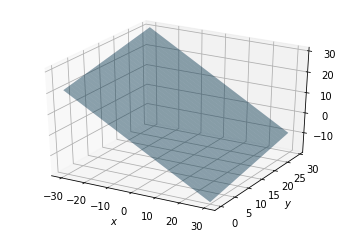
\includegraphics[width= \columnwidth]{figure4.png}
    \caption{Planes $P_1$ and $P_2$} \label{fig:1}
\end{figure}
\end{document}